\documentclass[a4paper]{article}

\usepackage{xcolor}
\usepackage{fancyheadings}
\usepackage{listings}
\usepackage{graphicx}
\usepackage[section]{placeins}
\usepackage{hyperref}
\usepackage[utf8]{inputenc}

% colors
\definecolor{mygreen}{rgb}{0,0.6,0}
\definecolor{mygray}{rgb}{0.5,0.5,0.5}
\definecolor{myblue}{rgb}{0,0,0.5}
\definecolor{mymauve}{rgb}{0.58,0,0.82}

% hyperref configuration
\hypersetup{
    colorlinks,
    linkcolor={mymauve},
    citecolor={myblue},
    urlcolor={myblue}
}

% Code listing configuration
\lstset{
  basicstyle=\footnotesize,        % the size of the fonts that are used for the code
  commentstyle=\color{mygreen},    % comment style
  keepspaces=true,                 % keeps spaces in text, useful for keeping indentation of code (possibly needs columns=flexible)
  keywordstyle=\color{blue},       % keyword style
  language=Python,                 % the language of the code
  morekeywords={interface,abstract,static}, % if you want to add more keywords to the set
  %numbers=left,                    % where to put the line-numbers; possible values are (none, left, right)
  numbersep=5pt,                   % how far the line-numbers are from the code
  numberstyle=\tiny\color{mygray}, % the style that is used for the line-numbers
  stringstyle=\color{mymauve}      % string literal style
}

% TODO command
\newcommand{\todo}[1]{\textcolor{red}{[#1]}\\}

% New custom label command
\makeatletter
\newcommand{\customlabel}[2]{%
   \protected@write \@auxout {}{\string \newlabel {#1}{{#2}{\thepage}{#2}{#1}{}} }%
   \hypertarget{#1}{#2}
}
\makeatother

% requirements
\newcounter{reqcount}
\newcommand{\requirement}[2]{%
  \item \refstepcounter{reqcount}\customlabel{req:#1}{\textbf{Eis \thereqcount}}: #2
}

\newcommand{\reqref}[1]{\ref{req:#1}}

% questions
\newcommand{\question}[1]{
  \subsubsection*{#1}
  \pdfbookmark[2]{#1}{question:#1}
}

% code in text
\newcommand{\code}[1]{\lstinline[columns=fixed]{#1}}

% heading
\lhead{Open Universiteit}
\chead{IM0102, Design patterns}
\rhead{Eindopdracht}

\begin{document}
\pagestyle{fancy}

\section*{Studentgegevens}
    \begin{description}
        \item [Cursuscode] IM0102
        \item Jabberpoint Inhoudsopgave
        \item [Naam] Daniel S. C. Schiavini
        \item [Studentnummer] 851102873
    \end{description}

\section*{Aanpak}
    De oorspronkelijke bedoeling was om deze opdracht uit te voeren in een team met een andere student.
    Echter, er was geen andere student beschikbaar met een vergelijkbare tempo.
    Daardoor heb ik deze opdracht alleen uitgevoerd.

    Voordat ik wist dat ik de opdracht alleen mag uitvoeren, heb ik een Git repository gemaakt.
    Ik heb de repository zo geconfigureerd dat dit document automatisch wordt gebouwd door het gebruik van TravisCI.
    Zodra een nieuwe versie van het rapport naar GitHub wordt gepushed, draait een script dat het PDF-bestand maakt.
    Het script bouwt ook Jabberpoint, draait unit tests, en als alles gelukt is wordt ook een JAR-bestand gemaakt.
    In de master branch hangt een deployment vast dat het PDF en JAR naar \href{https://github.com/DanielSchiavini/design-patterns-assignment/tree/gh-pages}{GitHub pages} publiceert.

    Jabberpoint had nog geen geautomatiseerde tests ingebouwd, en omdat ik dat belangrijk vind, heb ik van tevoren JUnit tests geschreven.
    Echter niet alle klassen waren testbaar - TravisCI draait in een Linux-container waarin de Graphic Java-klassen niet gecreëerd kunnen worden.
    Ik had niet genoeg tijd had om dit probleem op te lossen, daarom heb ik alleen tests geschreven voor de domein- en accessor-klassen.

\section{Probleemanalyse}
    \label{sec:probleemanalyse}
    Om het probleem te analyseren kunnen we het beste de opdracht in eisen omschrijven:

    \begin{itemize}
        \requirement{toevoegen}{De gebruiker moet één of meer slides met inhoudsopgaven kunnen toevoegen aan een presentatie.}
        \requirement{tonen}{Een inhoudsopgave-slide moet alle onderwerpen van de presentatie tonen.}
        \requirement{samenvoegen}{Het onderwerp moet slechts eenmaal worden getoond wanneer meerdere slides achter elkaar hetzelfde onderwerp hebben.}
        \requirement{updaten}{De inhoudsopgave moet automatisch worden geüpdatet wanneer slides worden toegevoegd of verwijderd.}
        \requirement{titel}{De titel moet als onderwerp worden gebruikt wanneer een slide geen onderwerp heeft (\textbf{aanname}).}
        \requirement{onderwerpen}{Het onderwerp mag op slides worden getoond, behalve in de inhoudsopgave (optioneel).}
        \requirement{volgnummers}{De onderwerpen in de inhoudsopgave mogen volgnummers krijgen (optioneel).}
        \requirement{aanduiding}{Het onderwerp van de slide die na een inhoudsopgave komt, mag een speciale aanduiding krijgen (i.e. een alternatieve letterstijl) (optioneel).}
        \requirement{stijl}{De stijl van de inhoudsopgave is vrij te bepalen.}
    \end{itemize}

    De opdracht om een inhoudsopgave te implementeren in Jabberpoint is best interessant.
    Om een inhoudsopgave te implementeren, is kennis nodig van de hele presentatie.
    Een verandering in elke slide kan invloed hebben op alle inhoudsopgaven.
    Deze circulaire afhankelijkheid maakt de opdracht uitdagend.

\section{Ontwerp}
    Het onderwerp zoals geïmplementeerd verandert weinig van het originele Jabberpoint-ontwerp.
    Er is een nieuwe klasse toegevoegd voor de inhoudsopgaven, namelijk \code{TableOfContentsSlide}.
    Deze nieuwe klasse is een sub-klasse van \code{Slide}.

    Het grootste verschil tussen de klassen is dat de inhoudsopgave kennis moet hebben van de hele presentatie.
    Daardoor krijgt een \code{TableOfContentsSlide} een referentie naar de presentatie in de constructor.

    Zodra de inhoudsopgave getekend gaat worden, worden de presentatie onderwerpen gelezen en wordt een nieuwe lijst van sub-items gemaakt.
    Daartoe kunnen wij de bestaande methoden van de \code{Slide} klasse gebruiken.
    Omdat er geen speciale stijl-eisen zijn voor de inhoudsopgave, kunnen wij eenvoudig de al ingebouwde levels gebruiken om de stijl te bepalen.

    De aangepaste klassendiagram wordt in figuur~\ref{fig:design} getoond.
    \begin{figure}[!htb]
     \caption{
        Klassendiagram voor de domein-objecten.\label{fig:design}
        Sterren geven de nieuwe klasse en methoden aan.
     }
     \centering 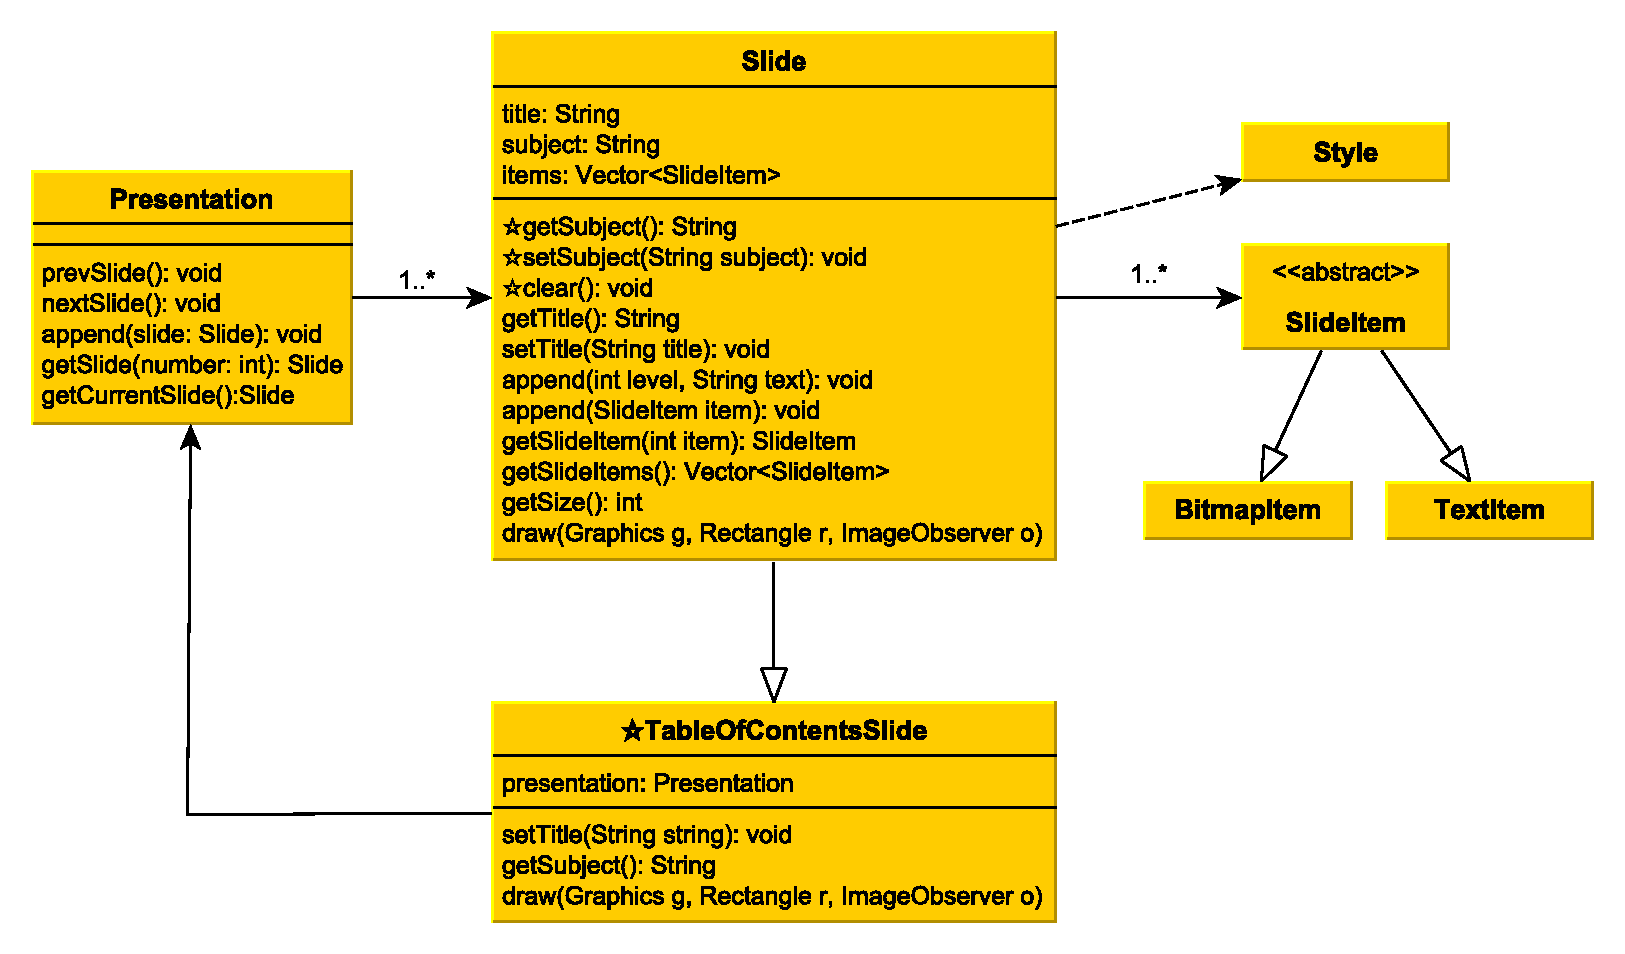
\includegraphics[width=\textwidth]{Diagrams/design.pdf}
    \end{figure}

    Het voordeel van dit onderwerp is dat er vrij weinig hoeft te veranderen.
    De Accessor-klassen krijgen de extra verantwoordelijkheid om de slide-objecten te maken en te schrijven.
    Voor de rest van de code is een inhoudsopgave een normale slide die zijn eigen content genereert.
    Accessor-klassen mogen zelf bepalen of er een referentie wordt opslagen naar een inhoudsopgave, of een lijst van de inhoud van de slides.

    Voor de implementatie van de \code{draw} methode was een manier nodig om alle eerdere slide-items te verwijderen.
    Het is natuurlijk ook mogelijk om de \code{items} attribuut rechtstreeks te veranderen;
    maar het is in Java nooit verstandig om attributen van andere klassen te veranderen.
    Daarvoor komt een nieuwe \textbf{protected} methode \code{clear} in de slide.
    De attributen van \code{Slide} zijn \textbf{private} geworden.

    Het is verstandig om software te implementeren in de meest simpele manier, en dan itereren om deze te verbeteren.
    Daarom vind ik dat het bij de opdracht past om een aantal verbeteringen ook door te voeren.
    Dit wordt verder uitgelegd in de volgende sectie.

    \subsection{Traceerbaarheid van eisen}
        In deze sectie geef ik onderdelen van het ontwerp aan die verantwoordelijk zijn om de eisen (zie sectie~\ref{sec:probleemanalyse}) te realiseren.
        Dit geeft dus de relatie tussen probleemanalyse en ontwerp.

        \begin{itemize}
            \item De \code{Accessor}-klassen zijn verantwoordelijk voor de volgende eisen: \reqref{toevoegen}.
            \item De \code{TableOfContentsSlide} klasse is verantwoordelijk voor: \reqref{tonen}, \reqref{samenvoegen},
                \reqref{updaten}, \reqref{titel}, \reqref{volgnummers}, \reqref{aanduiding} en \reqref{stijl}.
            \item De \code{Slide} klasse is verantwoordelijk voor: \reqref{onderwerpen}.
        \end{itemize}


\section{Keuzen}
    \question{Wanneer items genereren}
    \question{logic voor lezen van slides in presentatie?}
    \question{extract abstract from Slide class?}
    \question{toc te veel kennis van slide: misschien nieuwe slide maken en die laten tekenen? maar dan bij output heb je de items niet..}
    \question{refactoring van UI-domein vermengeling}
    \question{moet een inhoudsopgave verplicht een titel hebben?}
    \question{layouts i.p.v. draw}

\section{Sourcecode}
In deze sectie geef ik links naar de verschillende resultaten van de opdracht.
Alle links hebben betreft zowel op Jabberpoint als voor dit rapport.
\begin{itemize}
    \item Java en \LaTeX ~code:
        \hyperlink{https://github.com/DanielSchiavini/design-patterns-assignment}{github.com/DanielSchiavini/design-patterns-assignment}.
    \item Aanpassingen op Jabberpoint:
        \hyperlink{https://github.com/DanielSchiavini/design-patterns-assignment/compare/v0.0.1...master}{%
        github.com/DanielSchiavini/design-patterns-assignment/compare/v0.0.1...master}.
    \item Gegenereerde bestanden:
        \hyperlink{https://github.com/DanielSchiavini/design-patterns-assignment/tree/gh-pages}{github.com/DanielSchiavini/design-patterns-assignment/tree/gh-pages}
    \item Laatste build-rapport van TravisCI:
        \hyperlink{https://travis-ci.com/DanielSchiavini/design-patterns-assignment}{travis-ci.com/DanielSchiavini/design-patterns-assignment}
    \item Rapporten van TravisCI:
        \hyperlink{https://travis-ci.com/DanielSchiavini/design-patterns-assignment/builds}{travis-ci.com/DanielSchiavini/design-patterns-assignment/builds}
    \item Optionele implementaties:
        \hyperlink{https://github.com/DanielSchiavini/design-patterns-assignment/pulls}{github.com/DanielSchiavini/design-patterns-assignment/pulls}
\end{itemize}

\end{document}
